\subsection{Multi-Queue NICs}

So far we optimized \textbf{how one queue interacts with one single CPU core}. However, modern NICs have multiple queues, and we can use them to further increase the performance of the system. This section describes how to reach parallelism in the NIC and how to use it to further increase the performance of the system.

\highspace
\begin{flushleft}
    \textcolor{Red2}{\faIcon{exclamation-triangle} \textbf{Why single RX queue is not enough}}
\end{flushleft}
The simplest design is:
\begin{equation*}
    \text{NIC} \rightarrow \textbf{one RX queue} \rightarrow \text{one interrupt} \rightarrow \text{one CPU core}
\end{equation*}
Even with interrupt coalescing, pooling or NAPI, we still have a fundamental bottleneck: \textbf{one RX queue can effectively feed only one core at a time}.

\highspace
Modern servers have $8$/$16$/$32+$ CPU cores and $25$/$40$/$100$ Gbps NICs, and if all packets go through a single RX descriptor ring and a single interrupt source, then only one core does packet processing, and the rest of the cores are idle. This is a \textbf{per-core performance ceiling}\footnote{Ceiling means that no matter how much we optimize the system, we cannot go beyond a certain performance level}.

\highspace
\textcolor{Red2}{\faIcon{question-circle} \textbf{What breaks first?}} At high traffic rates, a single core becomes saturated and the RX ring fills up, causing \textbf{packet drops}. So the problem is no longer livelock (\autopageref{sec:the-receive-live-lock-problem}), but \textbf{lack of parallelism}.

\highspace
\begin{flushleft}
    \textcolor{Green3}{\faIcon{check-circle} \textbf{Solution: Hardware RX queues}}
\end{flushleft}
The solution is to \textbf{replicate the RX queue in hardware}. Modern NICs provide multiple \emph{independent} RX queues, each with:
\begin{itemize}
    \item Its own descriptor ring;
    \item Its own interrupt source;
    \item Its own NAPI context.
\end{itemize}
So the architecture becomes:
\begin{center}
    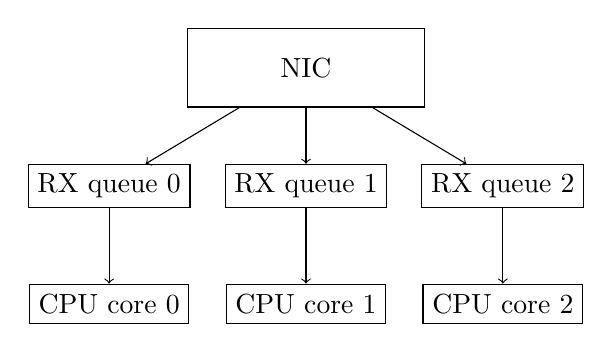
\begin{tikzpicture}[node distance=1.5cm, auto]
        % Nodes
        \node (nic) [draw, rectangle, minimum width=3cm, minimum height=1cm] {NIC};

        \node (rx0) [draw, rectangle, minimum width=2cm, minimum height=0.5cm, below of=nic, xshift=-2.5cm] {RX queue 0};
        \node (rx1) [draw, rectangle, minimum width=2cm, minimum height=0.5cm, below of=nic] {RX queue 1};
        \node (rx2) [draw, rectangle, minimum width=2cm, minimum height=0.5cm, below of=nic, xshift=2.5cm] {RX queue 2};
        
        \node (cpu0) [draw, rectangle, minimum width=2cm, minimum height=0.5cm, below of=rx0] {CPU core 0};
        \node (cpu1) [draw, rectangle, minimum width=2cm, minimum height=0.5cm, below of=rx1] {CPU core 1};
        \node (cpu2) [draw, rectangle, minimum width=2cm, minimum height=0.5cm, below of=rx2] {CPU core 2};
        
        % Arrows
        \draw[->] (nic) -- (rx0);
        \draw[->] (nic) -- (rx1);
        \draw[->] (nic) -- (rx2);
        \draw[->] (rx0) -- (cpu0);
        \draw[->] (rx1) -- (cpu1);
        \draw[->] (rx2) -- (cpu2);
    \end{tikzpicture}
\end{center}
Each queue operates independently and can feed a different CPU core, allowing for parallel packet processing.

\newpage

\noindent
\textcolor{Green3}{\faIcon{question-circle} \textbf{What changes physically?}} Instead of one RX descriptor ring in DRAM, we now have \textbf{multiple descriptor rings} and \textbf{multiple sets of packet buffers}. The NIC can decide which queue to use for each incoming packet, and the CPU cores can process packets from their assigned queues in parallel.

\highspace
\begin{flushleft}
    \textcolor{Green3}{\faIcon{cog} \textbf{Mapping queues to CPU cores}}
\end{flushleft}
Now comes an important design choice: \textbf{\emph{which CPU core should handle which RX queue?}} The simplest approach is to use a \textbf{static mapping}, where each RX queue is assigned to a specific CPU core (i.e., RX queue $i$ is handled by CPU core $i$). This is done via \textbf{CPU affinity} settings in the operating system.

\highspace
\begin{flushleft}
    \textcolor{Green3}{\faIcon{\speedIcon} \textbf{Concurrency and cache locality}}
\end{flushleft}
With multiple RX queues processing packets in parallel, there is no need for locking between cores or for contention over shared RX ring resources. Each queue is independent, so there are no shared data structures requiring synchronization. This architecture scales well with the number of CPU cores as long as the NIC has enough RX queues to match the number of cores. This is the \textbf{benefit of concurrency}.

\highspace
Furthermore, if packets from the same flow always go to the same RX queue and that queue is always handled by the same CPU core, we can \textbf{benefit from cache locality}. The TCP state stays in the same core's cache, the socket buffers stay warm, and there are fewer cache misses. However, if packets from one flow bounce across different cores, cache lines move between cores, and memory coherence traffic increases. This can \textbf{degrade performance}. Therefore, \textbf{multi-queue NICs only help if the queue-to-core mapping preserves locality} (i.e., packets from the same flow are processed by the same core).

\highspace
In summary, multi-queue NICs enable scalable packet processing by providing multiple independent receive queues that can be mapped to different CPU cores, allowing parallelism while preserving cache locality and reducing contention.